\section{Boltzmann Machines} 

\subsection{Graphical Models}
  Graphical models allow a nice way to represent complex probability distributions with some dependence relationship. 

  \subsubsection{Directed Graphical Models}

    \begin{definition}[Directed Probability Graph]  
    A \textbf{probability graph} is a directed acyclic graph of $M$ nodes representing a joint probability distribution of $M$ scalar random variables. An edge pointing $A \rightarrow B$ means that the $B$ is conditionally dependent on $A$, and that there is a very clear casual relationship coming from $A$ to $B$. 
    \begin{center}
      graphics need to be added
    \end{center}
    The \textbf{parents} of a node $x_i$ is denoted $\mathrm{pa}_i$, and the entire joint distribution can be broken up as such: 
    \[p(\mathbf{x}) = \prod_{m=1}^M p(x_m \mid x_{\mathrm{pa}_m})\]
    \end{definition}


    \begin{example}[Relay Race]
      TBD
    \end{example} 


    Bayesian modelling with hierarchical priors. 

    \begin{definition}[Ancestral Sampling] 
    We can sample from the joint distribution by sequentially sampling starting from the parents to the final children, and discarding the ones (marginalizing) that we don't wish to sample. 
    \end{definition}


    \begin{example}
    We first provide some motivation from a computational complexity perspective. Given a joint distribution of 2 random variables $\mathbf{x}_1, \mathbf{x}_2$, say which are multinomial with $K$ classes, their joint distribution $p(\mathbf{x}_1, \mathbf{x}_2)$ is captured by $K^2 - 1$ parameters. For a general $M$ random variables, then we have to keep a total of $K^M - 1$ parameters, and this increases exponentially. 
    \begin{center}
      TBD
    \end{center}
    By building a directed graph with say $r$ maximum number of variables appearing on either side of the conditioning bar in a single probability distribution, then the computational complexity scales as $O(K^r)$, which may save a lot of effort if $r << M$. 
    \end{example}

    Extending upon this example, we can see that we want to balance two things: 
    \begin{enumerate} 
      \item Fully conncted graphs have completely general distributions and have $O(K^M -1)$ number of parameters (too complex). 
      \item If there are no links, the joint distribution fully factorizes into the product of its marginals and has $M(K-1)$ parameters (too simple) . 
    \end{enumerate}
    Graphs that have an intermediate level of connectivity allow for more general distributions compared to the fully factorized one, while requiring fewer parameters than the general joint distribution. One model that balances this out is the hidden markov model. 

    \begin{example}[Chain Graph]
      Consider an $M$-node Markov chain. The marginal distribution $p(\mathbf{x}_1)$ requires $K-1$ parameters, and the remaining conditional distributions $p(\mathbf{x}_i \mid \mathbf{x}_{i-1})$ requires $K(K-1)$ parameters. Therefore, the total number of parameters is 
      \[K-1 + (M-1) (K-1) K \in O(M K^2)\]
      which scales relatively well, and we have 
      \[p(\{\mathbf{x}_m\}) = p (\mathbf{x}_1) \prod_{m=2}^M p(\mathbf{x}_m \mid \mathbf{x}_{m-1})\]
    \begin{center}
      TBD
    \end{center}
    We can turn this same graph into a Bayesian model by introducing priors for the paramters. Therefore, each node requires an additional parent representing the distribution over parameters (e.g. prior can be Dirichlet)  
    \[p(\{\mathbf{x}_m , \mu_m\}) = p(\mathbf{x}_1 \mid \mu_1) p(\mu_1) \prod_{m=2}^M p(\mathbf{x}_m \mid \mathbf{x}_{m-1}, \mu_m) p(\mu_m) \]
    with $p(\mu_m) = \mathrm{Dir}(\mu_m \mid \alpha_m)$ for some predetermined fixed hyperparameter $\alpha_m$. 
    \begin{center}
      \includegraphics[scale=0.5]{img/07_Boltzmann/dir_prior.png}
    \end{center}
    We could also choose to share a common prior over the parameters, trading flexibility for computational feasibility. 
    \begin{center}
      \includegraphics[scale=0.5]{img/07_Boltzmann/shared_dir_prior.png}
    \end{center}
    \end{example}

    Another way to make more compact representations is through parameterized models. For example, if we have to compute $p(y = 1 \mid \mathbf{x}_1, \ldots, \mathbf{x}_M)$, this in general has $O(K^M)$ parameters. However, we can obtain a more parsimonious form by using a logistic function acting on a linear combination of the parent variables 
    \[p(y = 1 \mid \mathbf{x}_1, \ldots, \mathbf{x}_m) = \sigma \bigg( w_0 + \sum_{i=1}^M w_i x_i \bigg) = \sigma(\mathbf{w}^T \mathbf{x}) \]
    We can look at an example how this is applied to sampling from high-dimensional Gaussian with \textbf{linear Gaussian models}.  


    \begin{example}[Multivariate Gaussian]
      Consider an arbitrary acyclic graph over $D$ random variables, in which eachnode represents a single continuous Gaussian distribution with its mean given by a linear function of its parents. 
      \[p(x_i \mid \mathbf{pa}_i) = N \bigg( x_i \bigg| w_{ij} x_j + b_j, v_i \bigg) \]
      Given a multivariate Gaussian, let us try to decompose it into a directed graph. The log of the joint distribution takes form 
      \[\ln p(\mathbf{x}) = \sum_{i=1}^D \ln p(x_i \mid \mathrm{pa}_i) = - \sum_{i=1}^D \frac{1}{2 v_i} \bigg( x_i - \sum_{j \in \mathrm{pa}_i} w_{ij} x_j - b_i \bigg)^2 + \mathrm{const}\]
      To compute the mean, we can see that by construction, every $x_i$ is dependent on its ancestors, so 
      \[x_i = \sum_{j \in \mathrm{pa}_i} w_{ij} x_j + b_i + \sqrt{v_i} \epsilon_i, \;\; \epsilon_i \sim N(0, 1)\]
      so by linearity of expectation, we have 
      \[\mathbb{E}[x_i] = \sum_{j \in \mathrm{pa}_i} w_{ij} \mathbb{E}[x_j] + b_i\]
      So again, we can start at the top of the graph and compute the expectation. To compute covariance, we can obtain the $i, j$th element of $\boldsymbol{\Sigma}$ with a recurrence relation: 
      \begin{align*} 
        \Sigma_{ij} & = \mathbb{E}[ (x_i - \mathbb{E}[x_i]) (x_j - \mathbb{E}[x_j])] \\
                    & = \mathbb{E} \bigg[ (x_i - \mathbb{E}[x_i]) \bigg( \sum_{k \in \mathrm{pa}_j} w_{j k} (x_k - \mathbb{E}[x_k])  + \sqrt{v_i} \epsilon_j\bigg) \bigg] \\
                    & = \sum_{k \in \mathrm{pa}_j} w_{j k} \Sigma_{ik} + I_{ij} v_j
      \end{align*}
      If there were no links in the graphs, then the $w_{ij}$'s are $0$, and so $\mathbb{E}[\mathbf{x}] = [b_1, \ldots, b_D]$, making the covariance diagonal.If the graph is fully connected, then the total number of parameters is $D + D(D-1)/2$, which corresponds to a general symmetric covariance matrix.  
    \end{example}

    \begin{example}[Bilinear Gaussian Model]
      Consider the following model
      \begin{align*}
        u & \sim N(0, 1) \\
        v & \sim N(0, 1) \\
        r & \sim N(u v, 1)
      \end{align*}
      where the mean of $r$ is a product of $2$ Gaussians. This is also a parameterized model. 
      \begin{center}
        \includegraphics[scale=0.6]{img/07_Boltzmann/bilinear_gaussian.png}
      \end{center}
    \end{example}

    \begin{definition}[Conditional Independence in Directed Graphs]
      We say that $a$ is independent of $b$ given $c$ if 
      \[p(a \mid b, c) = p(a \mid c)\]
      or equivalently, 
      \[p(a, b \mid c) = p(a \mid b, c)\, p(b \mid c) = p(a \mid c) \, p(b \mid c)\]
      Conveniently, we can directly read conditional independence properties of the joint distribution from the graph without any analytical measurements. 
    \end{definition}

    \begin{example}
      We can demonstrate conditional independence with iid data. Consider the problem of density estimation of some dataset $\mathcal{D} = \{x_i\}$ with some parameterized distribution of $\mu$. As shown below, if we condition on $\mu$ and considered the joint over the observed variables, the variables are independent, but if we integrate out $\mu$, the observations are no longer independent. 
      \begin{center}
        \includegraphics[scale=0.6]{img/07_Boltzmann/iid_conditional_independence.png}
      \end{center}
    \end{example}

    The example above identifies a node (the parent $\mu$) where, if observed, causes the rest of the nodes to become independent. We can extend on this idea by taking an arbitrary $x_i$ and finding a set of nodes such that if they are observed, then $x_i$ is indepedent from every other node. 

    \begin{definition}[Markov Blanket]
      The \textbf{Markov blanket} of a node is the minimal set of nodes that must be observed to make this node independent of all other nodes. It turns out that the parents, children, and coparents are all in the Markov blanket. 
      \begin{center}
        \includegraphics[scale=0.6]{img/07_Boltzmann/markov_blanket.png} 
      \end{center}
    \end{definition} 

    One final interpretation is that we can view directed graphs as \textbf{distribution filters}. We take the joint probability distribution, will starts off as fully connected, and the directed graphs ``filters" away the edges that are not needed. Therefore, the joint probability distribution $p(\mathbf{x})$ is only allows through the filter if and only if it satisfies the factorization property. 

  \subsubsection{Undirected Graphical Models}

    As the name implies, undirected models use undirected graphs, which are used to model relationships that go both ways rather than just one. Unlike directed graphs, which are useful for expressing casual relationships between random variables, undirected graphs are useful for expressing soft constraints between random variables.  

    \begin{definition}[Conditional Independence in Undirected Graphs]
      Fortunately, conditional independence is easier compared to directed models. We can say $A$ is conditionally independent to $B$ given $C$ if $C$ blocks all paths between any node in $A$ and any node in $B$. 
      \begin{center}
        \includegraphics[scale=0.4]{img/07_Boltzmann/conditional_independence_undirected.png}
      \end{center}
    \end{definition}

    \begin{definition}[Markov Blanket in Undirected Graphs]
      The Markov blanket of a node, which is the minimal set of nodes that must be observered to make this node independent of the rest of the nodes, is simply the nodes that are directly connected to that node. 
      \begin{center} 
        \includegraphics[scale=0.4]{img/07_Boltzmann/markov_blanket_undirected.png}
      \end{center}
      Therefore, the conditional distribution of $x_i$ conditioned on all the variables in the graph is dependent only on the variables in the Markov blanket. 
    \end{definition}

    Now, let us talk about how we can actually define a probability distribution with this graph. 

    \begin{definition}[Clique] 
      In an undirected graph, a \textbf{clique} is a set of nodes such that there exists a link between all pairs of nodes in that subset. A \textbf{maximal clique} is a clique such that it is not possible to include any other nodes in the set without it ceasing it to be a clique. 
    \end{definition}

    Given a joint random variable $\mathbf{x}$  represented by an undirected graph, the joint distribution is given by the product of non-negative potential functions over the maximal cliques 
    \[p(\mathbf{x}) = \frac{1}{Z} \prod_C \phi_C (x_C)\] 
    where 
    \[Z = \int p(\mathbf{x}) \,d\mathbf{x}\] 
    is the normalizing constant, called the \textbf{partition function}. That is, each $x_C$ is a maximal clique and $\phi_C$ is the nonnegative potential function of that clique. 

    This assignment looks pretty arbitrary. How do we know that any arbitrary joint distribution of $\mathbf{x}$, which has a undirected graphical representation, can be represented as the product of a bunch of functions over the maximum cliques? Fortunately, there is a mathematical result that proves this. 

    \begin{theorem}[Hammersley-Clifford] 
      The joint probability distribution of any undirected graph can be written as the product of potential functions on the maximal cliques of the graph. Furthermore, for any factorization of these potential functions, there exists an undirected graph for which is the joint.  
    \end{theorem} 


    \begin{example}
      For example, the joint distribution of the graph below
      \begin{center}
        \includegraphics[scale=0.5]{img/07_Boltzmann/clique_factor.png}
      \end{center}
      factorizes into 
      \[p(A, B, C, D) = \frac{1}{Z} \phi(A, C) \, \phi(C, B) \, \phi(B, D) \, \phi(A, D)\]
    \end{example}

    Note that each potential function $\phi$ is a mapping from the joint configuration of random variables in a clique to non-negative real numbers. The choice of potential functions is not restricted to having specific probabilistic interpretations, but since they must be nonnegative, we can just represent them as an exponential. The negative sign is not needed, but is a remnant of physics notation. 
    \[p (\mathbf{x}) = \frac{1}{Z} \prod_C \phi_C (x_C) = \frac{1}{Z} \exp \bigg\{ - \sum_C E(x_C) \bigg\} = \frac{1}{Z} \underbrace{\exp \big\{ - E(\mathbf{x}) \big\}}_{\substack{\text{Boltzmann}\\ \text{distribution}}}\]

    Any distribution that can be represented as the form above is called a \textbf{Boltzmann distribution}. So far, all we stated is that the joint probability distribution can be expressed as the product of a bunch of potential functions, but besides the fact that it is nonnegative, there is no probabilistic interpretation of these potentials (or equivalently, the energy functions). While this does give us greater flexibility in choosing potential functions, we must be careful in choosing them (e.g. choosing something like $x^2$ may cause the integral to diverge, making the joint not well-defined).

    Clearly, these potential functions over the cliques should express which configuration of the local variables are preferred to others. It should assign higher values to configurations that are deemed (either by assumption or through training data) to be more probable. That is, each potential is like an ``expert" that provides some opinion (the value) on a configuration, and the product of the values of all the potential represents the total opinion of all the experts. Therefore, global configurations with relatively high probabilities are those that find a good balance in satisfying the (possibly conflicting) influences of the clique potentials. 

    \begin{example}[Transmission of Colds] 
      Say that you want to model a distribution over three binary variables: whether you or not you, your coworker, and your roommate is sick ($0$ represents sick and $1$ represents healthy). Then, you can make simplifying assumptions that your roommate and your coworker do not know each other, so it is very unlikely that one of thme will give the other an infection such as a cold directly. Therefore, we can model the indirect transmission of a cold from your coworker to your roommate by modeling the transmission of the cold from your coworker to you and then you to your roommate. Therefore, we have a model of form

      \begin{center}
        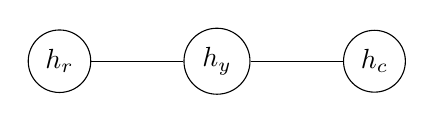
\begin{tikzpicture}
          \node[circle,draw] (hr) at (0,0) {$h_r$};
          \node[circle,draw] (hy) at (2,0) {$h_y$};
          \node[circle,draw] (hc) at (4,0) {$h_c$};

          \draw (hr) -- (hy);
          \draw (hy) -- (hc);
        \end{tikzpicture}
      \end{center}
      One max clique contains $h_y$ and $h_c$. The factor for this clique can be defined by a table and might have values resembling these. 

      \begin{table}[H]
        \centering
        \begin{tabular}{c|c|c|}
        \cline{2-3}
        & \( h_y = 0 \) & \( h_y = 1 \) \\ \hline
        \multicolumn{1}{|c|}{\( h_c = 0 \)} & 2 & 1 \\ \hline
        \multicolumn{1}{|c|}{\( h_c = 1 \)} & 1 & 10 \\ \hline
        \end{tabular}
        \caption{States and Values of \( h_y \) and \( h_c \)}
      \end{table}

      This table completely describes the potential function of this clique. Both of you are usually healthy, so the state $(1, 1)$ gets the maximum value of $1$. If one of you are sick, then it is likely that the other is sick as well, so we have a value of $2$ for $(0, 0)$. Finally, it is most unlikely that one of you is sick and the other healthy, which has a value of $1$. 
    \end{example}

\subsection{Boltzmann Machines} 

  Now that we've learned about graphical models, let's put them to use. We have some unknown joint distribution $\mathbf{x}$, and we want to represent it in a graph such that it is not too computationally hard to calculate probabilities and sample from them, but at the same time not so simple such that it doesn't richly capture a broad family of probability distributions. One architecture is to use \textbf{Markov Random Fields}, which represent these joint distributions with undirected graphs satisfying the Markov properties. 

  The Hammersley-Clifford theorem states that the joint PDF of any MRF can be written a a Boltzmann distribution. For now, we will limit outselves to \textbf{parwise MRFs}, which only capture dependencies between cliques of maximum size $2$. For example, a MRF can be represented with the graph $G(V, E)$ below. 
  \begin{center}
  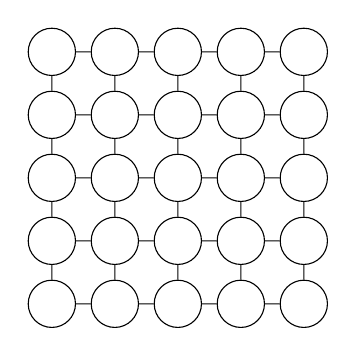
\begin{tikzpicture}[scale=0.8]
    % Define nodes in a 5x5 grid
    \foreach \i in {1,...,5} {
      \foreach \j in {1,...,5} {
        \node[circle, draw, minimum size=0.6cm] (node\i\j) at (\i, \j) {};
      }
    }

    % Connect nodes like an Ising model
    \foreach \i in {1,...,5} {
      \foreach \j in {1,...,5} {
        \pgfmathtruncatemacro{\right}{\i+1}
        \pgfmathtruncatemacro{\down}{\j-1}
        \pgfmathtruncatemacro{\up}{\j+1}
        \pgfmathtruncatemacro{\left}{\i-1}
        
        \ifnum \i < 5
          \draw (node\i\j) -- (node\right\j);
        \fi
        
        \ifnum \j > 1
          \draw (node\i\j) -- (node\i\down);
        \fi
      }
    }
  \end{tikzpicture}
  \end{center}

  \begin{definition}[Bernoulli Pairwise Markov Random Fields]
    MRFs with binary variables are sometimes \textbf{Ising models} in statistical mechanics, and \textbf{Boltzmann machines} in machine learning. By Hammersley-Clifford, we don't even need to specify the individual functions over the maximal cliques, and rather we can just specify the energy function $E(\mathbf{x})$ of the Boltzmann distribution that the MRF encodes. We define it to capture the interactions between random variables $x_i$ up to order $2$. 
      \[p_{\boldsymbol{\theta}} (\mathbf{x}) = \frac{1}{Z} \exp \bigg( \sum_{ij \in E} x_i x_j \theta_{ij} + \sum_{i \in V} x_i \theta_i \bigg) \]
    Now let's check its conditional distribution. 
      \begin{align*}
        p(x_k = 1 \mid \mathbf{x}_{-k}) & = \frac{p(x_k = 1, \mathbf{x}_{-k})}{p(\mathbf{x}_{-k})} \\
                                        & = \frac{p(x_k = 1, \mathbf{x}_{-k})}{p(x_k = 0, \mathbf{x}_{-k}) + p(x_k = 1, \mathbf{x}_{-k})} \\
                                        & = \frac{\exp \Big( \sum_{k j \in E} x_j \theta_{kj} + x_k \theta_k \Big)}{\exp(0) + \exp \Big(\sum_{k j \in E} x_j \theta_{kj} + x_k \theta_k \Big)} \\
                                        & = \sigma \bigg\{ - \theta_k x_k - \sum_{k j \in E} x_j \theta_{k j} \bigg\} 
      \end{align*}
    where the penultimate step comes from evaluating 
      \begin{align*} 
        p(x_k = 1, \mathbf{x}_{-k}) & = \frac{1}{Z(\boldsymbol{\theta})} \exp \bigg( \sum_{ij \in E, k \neq i, j} x_i x_j \theta_{ij} + \sum_{i j \in E, k = i, j} x_i x_j \theta_{ij} + \sum_{i \in V, i \neq k} x_i \theta_i + x_k \theta_k \bigg) \\
                                    & =\frac{1}{Z(\boldsymbol{\theta})} \exp \bigg( \sum_{ij \in E, k \neq i, j} x_i x_j \theta_{ij} + \sum_{k j \in E} x_j \theta_{kj} + \sum_{i \in V, i \neq k} x_i \theta_i + \theta_k \bigg)  \\ 
        p(x_k = 0, \mathbf{x}_{-k}) & = \frac{1}{Z(\boldsymbol{\theta})} \exp \bigg( \sum_{ij \in E, k \neq i, j} x_i x_j \theta_{ij} + \sum_{i \in V, i \neq k} x_i \theta_i\bigg)  
      \end{align*}
    and canceling out like terms in the numerator and denominator. This tells us that MRFs are related to logistic function.  
  \end{definition}

  We have given our first example of a Boltzmann machine. Let's generalize this a little bit by removing the restriction that there can only be pairwise connections. Then, we can model the second order interactions with the slightly more generalized energy function
    \[E(\mathbf{x}) = -\mathbf{x}^T \mathbf{U} \mathbf{x} - \mathbf{b}^T \mathbf{x}\]
  Now this slightly expands the coverage of probability distributions given our model, and we can see that this allows us to model Gaussian distributions. 

  \begin{example}[Gaussian Markov Random Fields] 
    If we assume that $p_{\boldsymbol{\theta}} ( \mathbf{x})$ folows a multivariate Gaussian distribution, we have 
      \[p(\mathbf{x} \mid \boldsymbol{\mu}, \boldsymbol{\Sigma}) = \frac{1}{Z} \exp \bigg( -\frac{1}{2} (\mathbf{x} - \boldsymbol{\mu})^T \boldsymbol{\Sigma}^{-1} (\mathbf{x} - \boldsymbol{\mu}) \bigg)\]
    Since the Gaussian distribution reprsents at most second-order relationships, it automatically encodes a pairwise MRF. Therefore, we can rewrite 
      \[p(\mathbf{x}) = \frac{1}{Z} \exp \bigg( -\frac{1}{2} \mathbf{x}^T J\mathbf{x} + \mathbf{g}^T \mathbf{x} \bigg)\] 
    where $J = \boldsymbol{\Sigma}^{-1}$ and $\boldsymbol{\mu} = J^{-1} \mathbf{g}$. 
  \end{example}

  Let's review what we had so far. There is a random vector $\mathbf{x}$ for which we would like to model the probability distribution of. 

  \begin{center}
    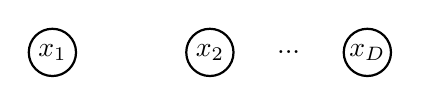
\begin{tikzpicture}
      % Define the nodes
      \node (x1) at (0,0) {$x_1$};
      \node (x2) at (2,0) {$x_2$};
      \node (xD) at (4,0) {$x_D$};

      % Add the "..." text box
      \node at (3,0) {...};
      \draw[thick] (x1) circle (0.3);
      \draw[thick] (x2) circle (0.3);
      \draw[thick] (xD) circle (0.3);
    \end{tikzpicture}
  \end{center}

  What we can do is model the dependencies between these random elements with linear parameters $\mathbf{W}$ and $\mathbf{b}$, which essentially gives us a Markov Random Field.  

  However, this is still quite a limited model. For one, due to the linearity of the weight matrix, it always turns out that the probability of $x_k = 1$ is always given by a linear model (logistic regression) from the values of the other units. This family of distributions parameterized by $\boldsymbol{\theta} = \{\mathbf{W}, \mathbf{b}\}$ may not be broad enough to capture the true $p(\mathbf{x})$. Therefore, we can add latent variables that can act similarly to hidden uits in a MLP and model higher-order interactions among the visible units. Just as the addition of hidden units to convert logistic regression into MLP results in the MLP being a universal approximator of functions, a Boltzmann machine with hidden units is not longer limited to modeling linear relationships between variables. Instead, the Boltzmann machine becomes a universal approximator of probability mass functions over discrete random variables. 

  \begin{definition}[Boltzmann Machine]
    The original \textbf{Boltzmann machine} has the energy function 
      \[E(\mathbf{v}, \mathbf{h}) = - \mathbf{v}^T \mathbf{R} \mathbf{v} - \mathbf{v}^T \mathbf{W} \mathbf{h} - \mathbf{h}^T \mathbf{S} \mathbf{h} - \mathbf{b}^T \mathbf{v} - \mathbf{c}^T \mathbf{h} \]
    It can represent the undirected graph that has connections within the $\mathbf{x}$, within the $\mathbf{h}$, and between the $\mathbf{x}$ and $\mathbf{h}$.
    \begin{center} 
      \includegraphics[scale=0.4]{img/07_Boltzmann/boltzmann_lateral.png}
    \end{center}
    Therefore, by adding latent variables and connecting everything together, this gives us a very flexible model that can capture a lot of distribtions.
  \end{definition} 

  \subsubsection{Restricted Boltzmann Machines} 

    \begin{definition}[Restricted Boltzmann Machine] 
      Now, if we put a restriction saying that there cannot be any intra-connections in the $\mathbf{x}$ and $\mathbf{h}$, then we get the \textbf{restricted Boltzmann machine}, which has a slightly more resticted form of the energy function than the general BM. The probability distributions that it can model has a graph that looks like 
      \begin{center}
        \includegraphics[scale=0.4]{img/07_Boltzmann/rbm_layer.png}
      \end{center}
      with connections only allowed between $x_i$'s and $h_j$'s, known as a \textbf{bipartite graph}, implying that the maximum clique length is $2$. This model allows the elements of $\mathbf{x}$ to be dependent, but this architecture allows for \textit{conditional independence}, and not just for $\mathbf{x}$ given $\mathbf{h}$, but also $\mathbf{h}$ given $\mathbf{x}$. Therefore, we already have the extremely nice property that 
      \begin{align*} 
        p(\mathbf{x} \mid \mathbf{h}) & = \prod_{k=1}^{D} p(x_k \mid \mathbf{h}) \\
        p(\mathbf{h} \mid \mathbf{x}) & = \prod_{j=1}^F p(h_j \mid \mathbf{x}) 
      \end{align*}
    \end{definition}

    The fact that we can calculate $p(\mathbf{h} \mid \mathbf{x})$ means that inferring the distribution over the hidden variables is easy. Keep in mind that there are three architectures we've talked about: 
    \begin{enumerate}
      \item Markov Random Fields, which model just the original $\mathbf{x}$. 
      \item Restricted Boltzmann machines, which models $\mathbf{x}, \mathbf{h}$ and not allowing intra-connections. 
      \item Boltzmann machines, which models $\mathbf{x}, \mathbf{h}$. Boltzmann machines without latent variables are just MRFs.  
    \end{enumerate}

    \begin{definition}[Bernoulli-Bernoulli RBM]
      For now, let us assume that we are trying to estimate the distribution of a Bernoulli random vector $\mathbf{x} \in \{0, 1\}^D$ with Bernoulli latent variables $\mathbf{h} \in \{0, 1\}^F$. Then, the energy of the joint configuration is  
        \[E(\mathbf{v}, \mathbf{h}; \boldsymbol{\theta}) = - \sum_{ij} W_{ij} v_i h_j - \sum_i b_i v_i - \sum_j a_j h_j = - \mathbf{v}^T \mathbf{W} \mathbf{h} - \mathbf{b}^T \mathbf{v} - \mathbf{a}^T \mathbf{h}\]
      where $\boldsymbol{\theta} = \{\mathbf{W}, \mathbf{a}, \mathbf{b}\}$ are the model parameters. So we have 
        \begin{align*} 
          p_{\boldsymbol{\theta}} (\mathbf{v}, \mathbf{h}) & = \frac{1}{Z} \exp \big( -E (\mathbf{v}, \mathbf{h}; \boldsymbol{\theta})\big) = \frac{1}{Z} \prod_{ij} e^{W_ij v_i h_j} \prod_i e^{b_i v_i} \prod_j e^{a_j h_j} \\
          Z & = \sum_{\mathbf{h}, \mathbf{v}} \exp \big( -E(\mathbf{v}, \mathbf{h}; \boldsymbol{\theta}) \big) 
        \end{align*}
      where we can think of the $\exp(\mathbf{h}^T \mathbf{W} \mathbf{x})$ as encoding the cliques of length $2$ and the others as cliques of length $1$.  
    \end{definition}

    Let's get some calculations out of the way. 

    \begin{lemma}[Conditional Distributions] 
      For the Bernoulli RBM, we have 
      \begin{align*} 
        p(h_j = 1 \mid \mathbf{x}) & = \sigma ( b_j + W_{j,:} \mathbf{x}) \\
        p(x_k = 1 \mid \mathbf{h}) & = \sigma ( c_k + \mathbf{h}^T \mathbf{W}_{:, k})
      \end{align*}
    \end{lemma}
    \begin{proof}
      Just use the definition of conditional probability and substitute the result below in the denominator. The terms will cancel out. 
    \end{proof}


    \begin{lemma}[Free Energy] 
      For the Bernoulli RBM, we want to compute the marginal $p(\mathbf{x})$ as
      \begin{align*} 
      p(\mathbf{x}) & = \frac{\exp(-F(\mathbf{x}))}{Z} \\
                    & = \frac{1}{Z} \exp \bigg( \mathbf{c}^T \mathbf{x} + \sum_{j=1}^H \log \big( 1 + \exp (b_j + \mathbf{W}_{j, :} \mathbf{x}) \big) \bigg) \\
                    & = \frac{1}{Z} \exp \bigg( \mathbf{c}^T \mathbf{x} + \sum_{j=1}^H \mathrm{softplus}(b_j + W_{j, :} \mathbf{x} ) \bigg)
      \end{align*}
      where $F$ is called the \textbf{free energy}. Therefore, $p(\mathbf{x})$ is calculated by taking the product of these terms, which is why it's known as a \textbf{product of experts model}. 
      \begin{center}
      \includegraphics[scale=0.4]{img/07_Boltzmann/softplus.png} 
      \end{center}
    \end{lemma}
    \begin{proof}
    We have 
    \begin{align*} 
      p(\mathbf{x}) & = \sum_{\mathbf{h} \in \{0, 1\}^H} \exp \big( \mathbf{h} \mathbf{W} \mathbf{x} + \mathbf{c}^T \mathbf{x} + \mathbf{b}^T \mathbf{h}\big) /Z \\
                    & = \exp (\mathbf{c}^T \mathbf{x}) \sum_{h_1 = 0, 1} \ldots \sum_{h_H = 0, 1} \exp \bigg( \sum_j h_j \mathbf{W}_{j, :} \mathbf{x} + b_j h_j \bigg) / Z \\
                    & = \exp (\mathbf{c}^T \mathbf{x}) \bigg( \sum_{h_1 = 0, 1} \exp (h_1 \mathbf{W}_{1, :} \mathbf{x} + b_1 h_1 ) \bigg) \ldots \bigg( \sum_{h_H = 0, 1} \exp (h_H \mathbf{W}_{H, :} \mathbf{x} + b_H h_H) \bigg) / Z \\
                    & = \exp (\mathbf{c}^T \mathbf{x}) \big( 1 + \exp (b_1 + \mathbf{W}_{1, :} \mathbf{x}) \big) \ldots \big( 1 + \exp (b_H + \mathbf{W}_{H, :} \mathbf{x})\big) / Z \\
                    & = \exp (\mathbf{c}^T \mathbf{x}) \exp\big\{ \log \big( 1 + \exp (b_1 + \mathbf{W}_{1, :} \mathbf{x}) \big) \big\} \ldots \exp \big\{ \log \big( 1 + \exp (b_H + \mathbf{W}_{H, :} \mathbf{x}) \big) \big\} / Z \\
                    & = \frac{1}{Z} \exp \bigg( \mathbf{c}^T \mathbf{x} + \sum_{j=1}^H \log \big( 1 + \exp (b_j + \mathbf{W}_{j, :} \mathbf{x}) \big) \bigg) 
    \end{align*} 
    \end{proof}

    Now that we've done this, we can finally get to training the model. Now, essentially this is density estimation problem given dataset $\mathcal{D} = \{\mathbf{x}^{(t)}\}$ of iid random variables, we want to maximize the likelihood of $p_{\boldsymbol{\theta}}$, which is really just equivalent to optimizing $E_{\boldsymbol{\theta}}$. So, let's take the average negative log-likelihood and take the derivative of it
    \[\frac{\partial}{\partial \boldsymbol{\theta}} \frac{1}{T} \sum_t - \log p_{\boldsymbol{\theta}} (\mathbf{x}^{(t)}) = \frac{1}{T} \sum_t - \log{p_{\boldsymbol{\theta}} (\mathbf{x}^{(t)})}\]
    There's a lot of computation to do here, so let's focus on one sample $\mathbf{x}^{(t)}$ and claim that the gradient ultimately ends up as the following. 

    \begin{theorem}
      It turns out that
      \begin{align*} 
      \frac{\partial}{\partial \boldsymbol{\theta}} - \log p(\mathbf{x}^{(t)}) & = \sum_{\mathbf{h}}  p(\mathbf{h} \mid \mathbf{x}^{(t)}) \, \frac{ \partial E(\mathbf{x}^{(t)}, \mathbf{h})}{\partial \boldsymbol{\theta}} - \sum_{\mathbf{x}, \mathbf{h}} p(\mathbf{x}, \mathbf{h}) \, \frac{\partial E(\mathbf{x}, \mathbf{h})}{\partial \boldsymbol{\theta}} \\
                                                                               & = \mathbb{E}_{\mathbf{h}} \bigg[ \frac{\partial E( \mathbf{x}^{(t)}, \mathbf{h})}{\partial \boldsymbol{\theta}} \; \bigg| \; \mathbf{x}^{(t)} \bigg] - \mathbb{E}_{\mathbf{x}, \mathbf{h}} \bigg[ \frac{\partial E(\mathbf{x}, \mathbf{h})}{\partial \boldsymbol{\theta}} \bigg]  
      \end{align*}
      The derivative of $E$ is easy since we already know the bilinear form by construction. In the left term, we are taking the expectation w.r.t. $p(\mathbf{h} \mid \mathbf{x}^{(t)})$, which we can factorize out due to conditional independence, so this is easy. However, the right term requires us to integrate over the joint $p(\mathbf{x}, \mathbf{h})$, which is intractable, and so we just approximate this with a Monte Carlo sample. 
    \end{theorem}
    \begin{proof}
      As a lemma, we first see that $\ln(Z) = \ln \big( \sum_{\mathbf{x}, \mathbf{h}} \exp \big( - E(\mathbf{x}, \mathbf{h}) \big) \big)$, and so
      \[\frac{\partial \ln(Z)}{\partial \boldsymbol{\theta}} = -\frac{1}{Z} \sum_{\mathbf{x}, \mathbf{h}} \exp \big(-E(\mathbf{x}, \mathbf{h})\big) \, \frac{E(\mathbf{x}, \mathbf{h})}{\partial \boldsymbol{\theta}} = - \sum_{\mathbf{x}, \mathbf{h}} p(\mathbf{x}, \mathbf{h}) \, \frac{\partial E(\mathbf{x}, \mathbf{h})}{\partial \boldsymbol{\theta}}\]
      We have 
      \begin{align*} 
      -\ln p(\mathbf{x}) & = - \ln \bigg\{ \sum_{\mathbf{h}} \exp \big( -E(\mathbf{x}, \mathbf{h}) \big) \bigg\} + \ln(Z)
      \end{align*}
      and so we can apply chain rule and multiply both numerator and denominator by $1/Z$ to get 
      \begin{align*} 
      -\frac{\partial}{\partial \boldsymbol{\theta}} \ln p(\mathbf{x}) & = \frac{\sum_{\mathbf{h}} \exp \big( -E(\mathbf{x}, \mathbf{h}) \big) \, \frac{\partial E(\mathbf{x}, \mathbf{h})}{\partial \boldsymbol{\theta}} / Z}{\sum_{\mathbf{h}} \exp \big( -E (\mathbf{x}, \mathbf{h}) \big) / Z} + \frac{\partial \ln(Z)}{\partial \boldsymbol{\theta}} \\
                                                                       & = \frac{\sum_{\mathbf{h}} p(\mathbf{x}, \mathbf{h}) \, \frac{\partial E(\mathbf{x}, \mathbf{h})}{\partial \boldsymbol{\theta}}}{p(\mathbf{x})} + \frac{\partial \ln(Z)}{\partial \boldsymbol{\theta}} \\
                                                                       & = \sum_{\mathbf{h}} p(\mathbf{h} \mid \mathbf{x}) \, \frac{\partial E(\mathbf{x}, \mathbf{h})}{\partial \boldsymbol{\theta}} - \sum_{\mathbf{x}, \mathbf{h}} p(\mathbf{x}, \mathbf{h}) \, \frac{\partial E(\mathbf{x}, \mathbf{h})}{\partial \boldsymbol{\theta}} 
      \end{align*}
    \end{proof} 

    So to calculate the second expectation, we can use a Gibbs sampler to do some numerical integration, but before we do that, let's just find the partial of $E$, which should be simple. 
    \[\frac{\partial E(\mathbf{x}, \mathbf{h})}{\partial W_{j k}} = \frac{\partial}{\partial W_{j k}} \bigg( - \sum_{j k} W_{j k} h_j x_k - \sum_k c_k x_k - \sum_j b_j h_j \bigg) = h_j x_k\]
    and so 
    \[\mathbb{E}_{\mathbf{h}} \bigg[ \frac{\partial E(\mathbf{x}, \mathbf{h})}{\partial W_{j k}} \bigg| \mathbf{x} \bigg] = \mathbb{E}_{\mathbf{h}} [ -h_j x_k \mid \mathbf{x}] = \sum_{h_j = 0, 1} - h_j x_k \, p(h_j \mid \mathbf{x}) = - x_k p(h_j = 1 \mid \mathbf{x})\]
    where the final term is a sigmoid. Hence, we have 
    \[\mathbb{E}_{\mathbf{h}} [ \nabla_{\mathbf{W}} E(\mathbf{w}, \mathbf{h}) \mid \mathbf{x}] = - \mathbf{h}(\mathbf{x}) \mathbf{x}^T, \text{ where } \mathbf{h}(\mathbf{x}) \coloneqq \begin{pmatrix} p(h_1 = 1 \mid \mathbf{x}) \\ \vdots \\ p(h_H = 1 \mid \mathbf{x}) \end{pmatrix} = \sigma(\mathbf{b} + \mathbf{W} \mathbf{x}) \]
    Now we can substitute what we solved into the second expectation, but again this is infeasible to calculate 
    \[\mathbb{E}_{\mathbf{x}, \mathbf{h}} \bigg[ \frac{\partial E(\mathbf{x}, \mathbf{h})}{\partial\boldsymbol{\theta}}\bigg] = \sum_{\mathbf{x}, \mathbf{h}} \mathbf{h}(\mathbf{x}) \mathbf{x}^T p(\mathbf{x}, \mathbf{h}) \]
    The way we do this is through \textbf{contrastive divergence}, which estimates the expectation through Gibbs sampling. Since we know $p(\mathbf{x}\mid \mathbf{h})$ and $p(\mathbf{h} \mid \mathbf{x})$ easily, we can start sampling the chain for some predetermined $K$ steps (actually $2K$ since we are sampling the $x$ and $h$ back and forth), and whatever $\bar{\mathbf{x}}$ you sample at the end is your estimate. So, once you should update your gradient, you start at the sample $\mathbf{x}^{(t)}$, run Gibbs for $k$ steps, and use that to estimate your gradient, and then move onto the next sample. We can tweak this procedure, such as \textbf{persistent CD}, where instead of initializing the chain to $\mathbf{x}^{(t)}$, we can initialize the chain to the negative sample of the last iteration. 
    \begin{center}
      \includegraphics[scale=0.4]{img/07_Boltzmann/contrastive_divergence.png}
    \end{center}
    Therefore, for updating $\mathbf{W}$, we get the following 
    \begin{align*} 
      \mathbf{W} & = \mathbf{W} - \alpha \big( \nabla_{\mathbf{W}}(- \log p(\mathbf{x}^{(t)})) \big) \\
                 & = \mathbf{W} - \alpha \big( \mathbb{E}_{\mathbf{h}} [ \nabla_{\mathbf{W}} E(\mathbf{x}^{(t)}, \mathbf{h}) \mid \mathbf{x}^{(t)} ] - \mathbb{E}_{\mathbf{x}, \mathbf{h}} [\nabla_{\mathbf{W}} E(\mathbf{x}, \mathbf{h}) ]\big) \\
                 & = \mathbf{W} - \alpha \big( \mathbb{E}_{\mathbf{h}} [ \nabla_{\mathbf{W}} E(\mathbf{x}^{(t)}, \mathbf{h}) \mid \mathbf{x}^{(t)} ] - \mathbb{E}_{\mathbf{h}} [\nabla_{\mathbf{W}} E(\bar{\mathbf{x}}, \mathbf{h}) \mid \bar{\mathbf{x}} ]\big) \\
                 & = \mathbf{W} + \alpha \big( \mathbf{h}(\mathbf{x}^{(t)}) (\mathbf{x}^{(t)})^T               - \mathbf{h}(\bar{\mathbf{x}}) \bar{\mathbf{x}}^T \big)
    \end{align*}
    and doing this over all three parameters leads to 
    \begin{align*} 
      \mathbf{W} & \leftarrow \mathbf{W} + \alpha \big( \mathbf{h} (\mathbf{x}^{(t)}) (\mathbf{x}^{(t)})^T - \mathbf{h}(\bar{\mathbf{x}}) \bar{\mathbf{x}}^T \big) \\
      \mathbf{b} & \leftarrow \mathbf{b} + \alpha \big( \mathbf{h}(\mathbf{x}^{(t)}) - \mathbf{h}(\bar{\mathbf{x}}) \big) \\
      \mathbf{c} & = \leftarrow \mathbf{c} + \alpha \big( \mathbf{x}^{(t)} - \hat{\mathbf{x}} \big) 
    \end{align*}
    Therefore, contrastive divergence with $k$ iterations gives us the \textbf{CD-k algorithm}. In general, the bigger $k$ is, the less biased the estimate of the gradient will be, and in practice $k=1$ works well for learning good features. The reason this is called contrastive divergence is that in the gradient update step, we have a positive sample and a negative sample that both approximates the expected gradient, which constrasts to each other. 

  \subsubsection{Gaussian Bernoulli RBMs}

    Now we can talk about Gaussian Bernoulli RBMs. 

    \begin{definition}[Gaussian-Bernoulli RBM] 
      If we assume that $\mathbf{v}$ is a real-valued (unbounded) input that follows a Gaussian distribution (with $\mathbf{h}$ still Bernoulli), then we can add a quadratic term to the energy function 
      \begin{equation} 
        E(\mathbf{x}, \mathbf{h}) = - \mathbf{h}^T \mathbf{W} \mathbf{x} - \mathbf{c}^T \mathbf{x} - \mathbf{b}^T \mathbf{h} - \frac{1}{2} \mathbf{x}^T \mathbf{x}
      \end{equation}
      In this case, $p(\mathbf{x} \mid \mathbf{h})$ becomes a Gaussian distribution $N(\mathbf{c} + \mathbf{W}^T \mathbf{h}, \mathbf{I})$. The training process is slightly harder for this, so what we usually do is normalize the training set by subtracting the mean off each input and dividing the input by the training set standard deviation to get  
      \begin{equation} 
        E(\mathbf{v}, \mathbf{h}; \boldsymbol{\theta}) = \sum_i \frac{(v_i - b_i)^2}{2 \sigma_i^2} - \sum_{ij} W_{ij} h_j \frac{v_i}{\sigma_i} - \sum_j a_j h_j
      \end{equation}
      You should also use a smaller learning rate $\alpha$ compared to Bernoulli RBM. 
    \end{definition} 

